\subsection{EXO-UL7}
\label{exo:exo-ul7}

keywords: model-based control; strength augmentation;\\

\begin{figure}[ht]
  \centering
  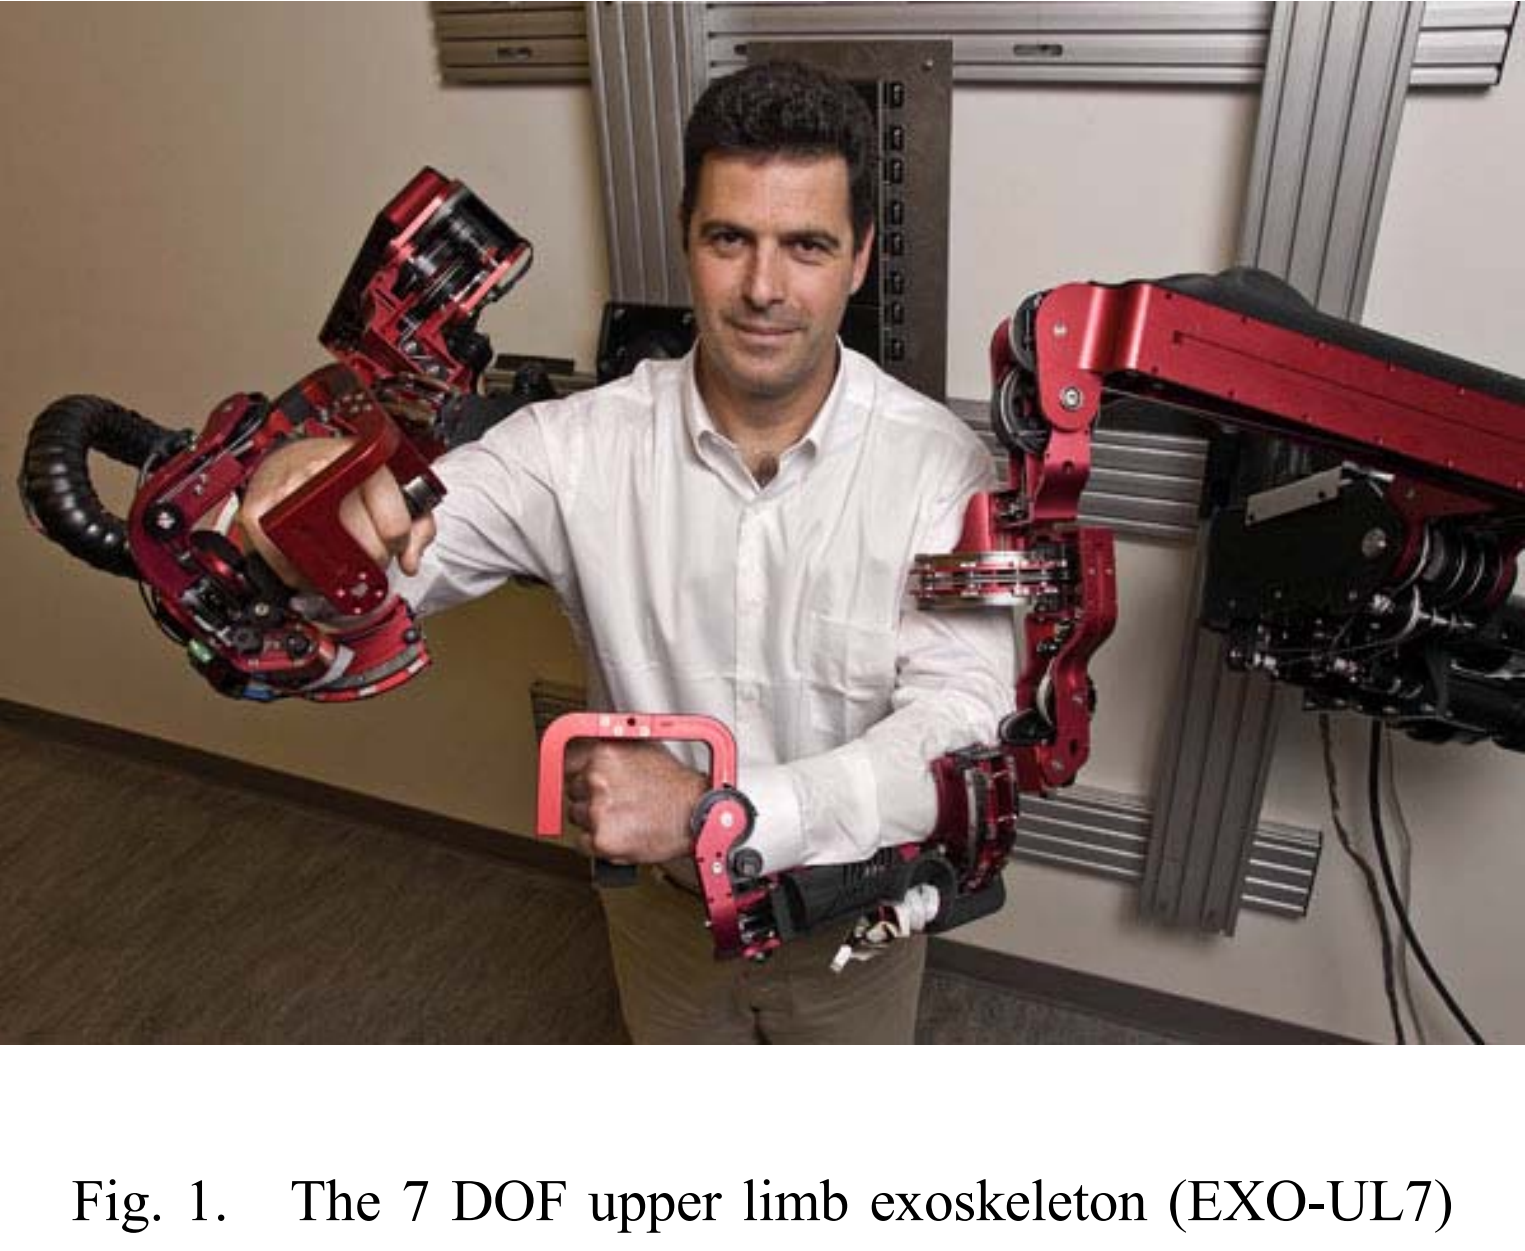
\includegraphics[width=4.0in]{exos/figs/exo-ul7.png}
\end{figure}


Although this study focuses on lower-body exoskeltons, we include the EXO-UL7 7 DOF upper-extremity exoskeleton for its novel actuation scheme and principled design. 

-------------------------------------------------

(Called CADEN - "cable driven dexterous exoskeleton for neurorehabilitation" in [[EXOul7design]])

Design:

7 DOF model; cable-actuated; proximal motor placement and distal cable-pulley reductions for low inertia, high stiffness links with backdrivable transmissions with zero backlash.  "Enables full glenohumeral, elbow, and wrist joint functionality." -- [[EXOul7design]]

% set the Human Machine Interface (HMI) at the neuromuscular level ... as one of the primary command signals... Use sEMG signals.  -- http://bionics.seas.ucla.edu/research/exoskeleton_device_3.html

[[EXOul7design]] contains data from a dynamic / kinematic study of human motion during everyday tasks in order to determine design requirements for exo.

3 lvls of safety mechanisms: 1) built in mechanical -- phys. stops, 2) electrical -- three wearer e-stops including an observer e-stop, an enable button which must be held, and a foot switch e-stop, and 3) software -- redundant position sensing (pots, Midori, Fullerton; shaft encoder, HP), one at either side of power train, monitor both joint motion and motor position. -- [[EXOul7design]]

Control bandwidth -- targeted 10Hz based on achievable frequency range of human arm which is btwn 2Hz and 5Hz.  They found shoulder joint had 1st resonant mode at 6 Hz. -- [[EXOul7design]]

Weight: 3.5 and 6kg from links 1 and links 2-7 (resp.). -- [[EXOul7design]]

Articulation: 7 single axis revolute joints.  Use three pulleys (90 and 180 deg configurations) at joints to keep cable length constant. Stack of pulleys required -- two pulleys representing agonist muscle groups and two for antagonist -- [[EXOul7design]]

Singularities: Design movable joint mechanisms that allow adjustment of singularity within 15deg based on user preferences. -- [[EXOul7design]]

Power transmission: shafts, cables, fluid lines, and gear trains.  Use pulleys for speed reductions and backdrivability.  2-stage pulleys in proximal joints 1-4 and single stage for more distal (5-7). -- [[EXOul7design]]

Motors for joints 1–4 were mounted on the stationary base, achieving a 60% reduction in overall weight of the moving parts. The remaining three motors, whose torque requirements are substantially less, were positioned on the forearm -- [[EXOul7design]]


Control Strategy:

Model-based control -- "proposed HMI takes advantage of the electro-chemical-mechanical delay, which inherently exists in the musculoskeletal system, between the time when the neural system activates the muscular system and the time when the muscles generate moments around the joints. The myoprocessor is a model of the human muscle running in real-time and in parallel to the physiological muscle.   During the electro-chemical-mechanical time delay, the system will gather information regarding the physiological muscle’s neural activation level based on processed sEMG signals, the joint position, and angular velocity, and will predict using the myoprocessor the force that will be generated by the muscle before physiological contraction occurs. By the time the human muscles contract, the exoskeleton will move with the human in a synergistic fashion, allowing natural control of the exoskeleton as an extension of the operator's body." %-- http://bionics.seas.ucla.edu/research/exoskeleton_device_3.html

Say they use neuro control strategy to avoid having to trigger motion based on human movement / force (required in position, force-impedance control) -- [[EXOul7design]]


References:

Cavallaro E., J. Rosen, J. C. Perry, S. Burns, B. Hannaford, Hill Based Model as a Myoprocessor for a Neural Controlled Powered Exoskeleton Arm – Parameter Optimization, Proceedings of the 2005 IEEE international Conference on Robotics and Automation, ICRA 2005, pp. 4525 – 4530, Barcelona Spain, April 2005

Rosen J,, J. C. Perry, N. Manning, S. Burns, B. Hannaford, The Human Arm Kinematics and Dynamics During Daily Activities – Toward a 7 DOF Upper Limb Powered Exoskeleton, - ICAR 2005 – Seattle WA, July 2005. [ CP19]

Perry J.C., J. Rosen, Design of a 7 Degree-of-Freedom Upper-Limb Powered Exoskeleton Proceedings of the 2006 BioRob Conference, Pisa, Italy, February, 2006.

Cavallaro E., J. Rosen, J. C. Perry, S. Burns, Myoprocessor for Neural Controlled Powered Exoskeleton Arm, IEEE Transactions on Biomedical Engineering, pp. 2387-2396, Vol. 53, No. 11, November 2006

Perry J. C., J. Rosen, S. Burns, Upper-Limb Powered Exoskeleton Design, IEEE Transactions on Mechatronics, Volume 12, No. 4, pp. 408-417, August 2007 <<EXOul7design>>

Rosen J., and J.C. Perry, Upper Limb Powered Exoskeleton, Journal of Humanoid Robotics, Vol. 4, No. 3 (2007) 1–20

Miller, L.M. and J. Rosen, 2010." Comparison of multi-sensor admittance control in joint space and task space for a seven degree of freedom upper
limb exoskeleton," 3rd IEEE RAS and EMBS International Conference on Biomedical Robotics and Biomechatronics (BioRob). <<EXOul7admitJointTaskCmp>>

Wen, Y., J. Rosen, and L. Xiaoou, 2011." PID admittance control for an upper limb exoskeleton," American Control Conference (ACC).  <<EXOul7admit>>

-------------------------------------------------

\subsection{Assessment and Recommendations}

The EXO-UL7 is a well-designed upper body exosekelton that is experimenting with new sEMG based control mechanisms.  The control approach is not as refined and needs to be developed further before field applications due to reliance on sEMG data.  
% As mentioned in Sections~\ref{exo:bleex} and \ref{exo:hal}, there are advantages to .


The figures in this section were obtained from \cite{EXOul7design2007,EXOul7pidAdmit2011}.  Materials presented are based on the references above.